\documentclass{standalone}

\begin{document}
\begin{figure*}
  \caption{\label{fig:earthsample}
    Sample image used to test the application of a generated lensing map.
  }
  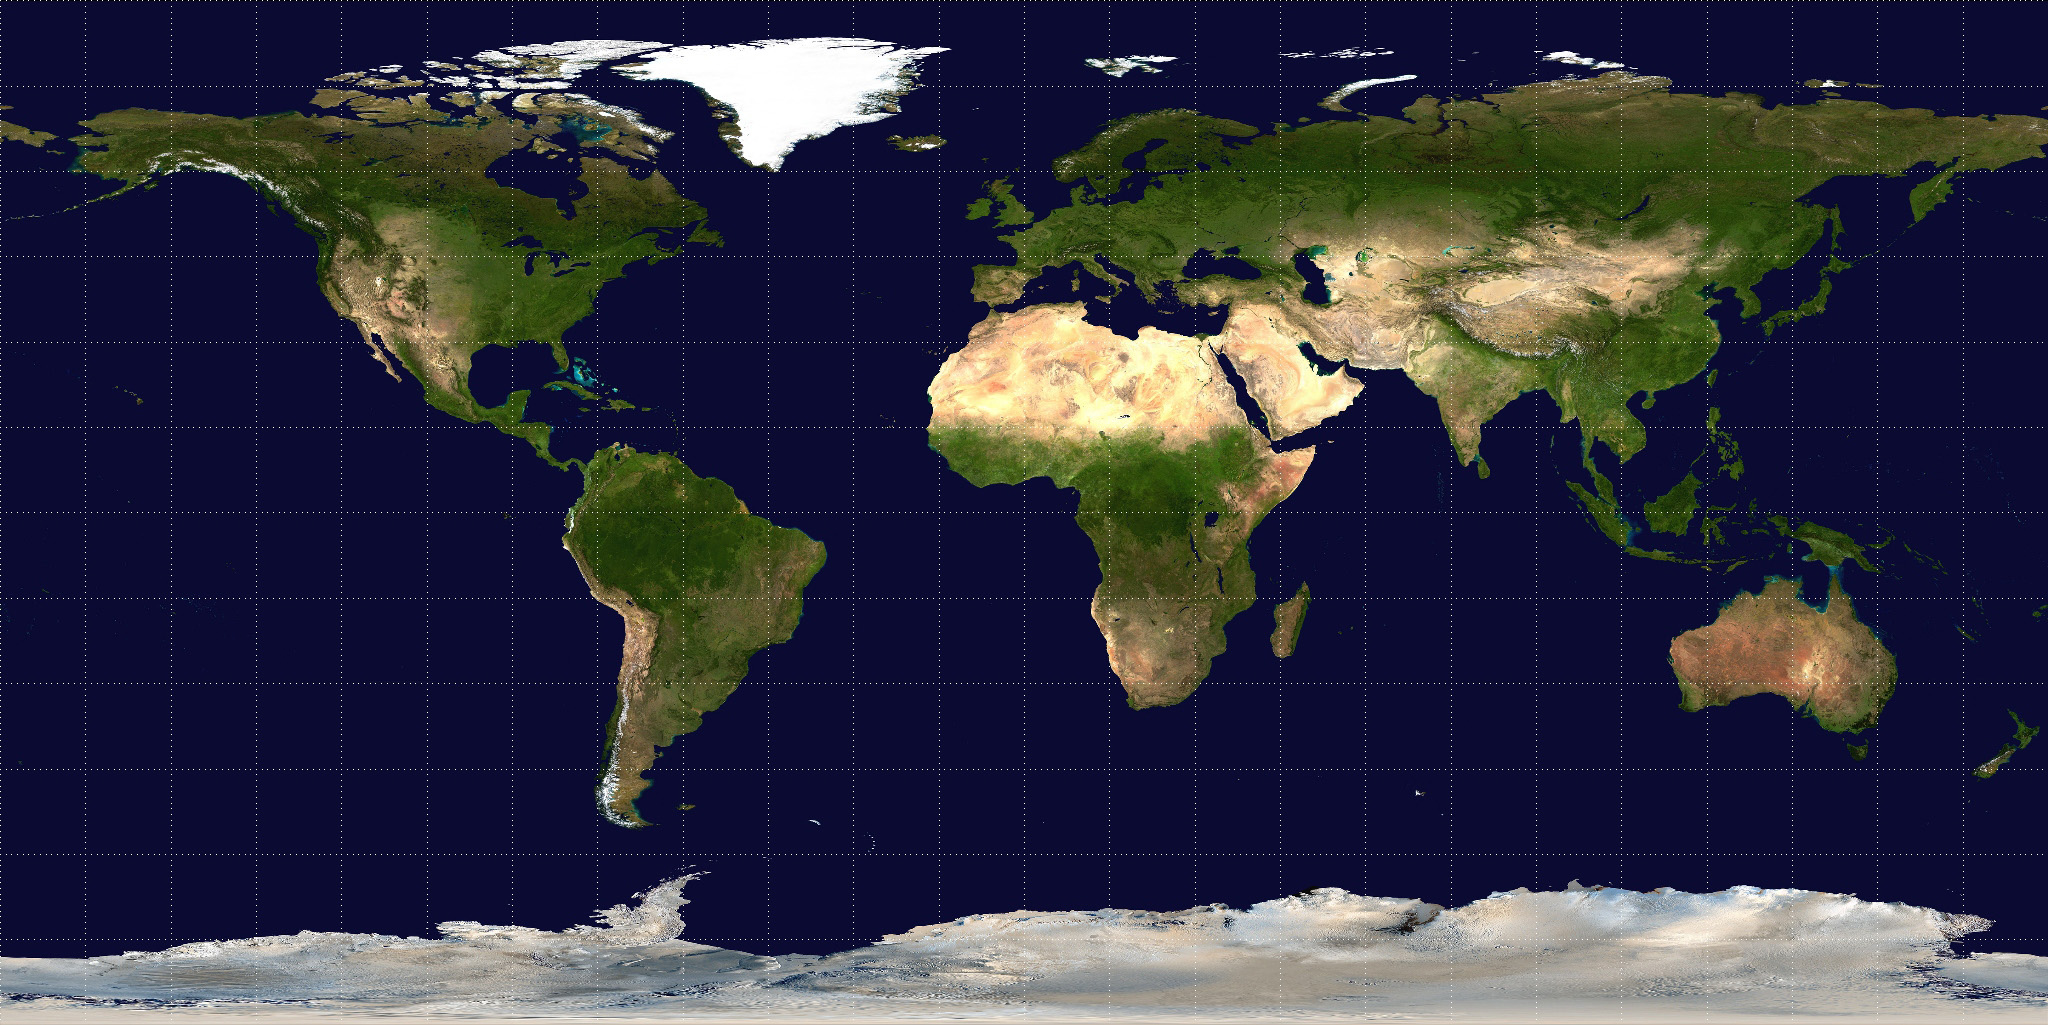
\includegraphics[width=\textwidth]{earth}
\end{figure*}

\begin{figure*}
  \caption{\label{fig:example1}
    Final result of applying the explicit Schwarzschild lensing map on the sample image shown in Fig.~(\ref{fig:earthsample}), with $M=\SI{1}{\kilo\meter}$ and $R_O=\SI{10}{\kilo\meter}$.
  }
  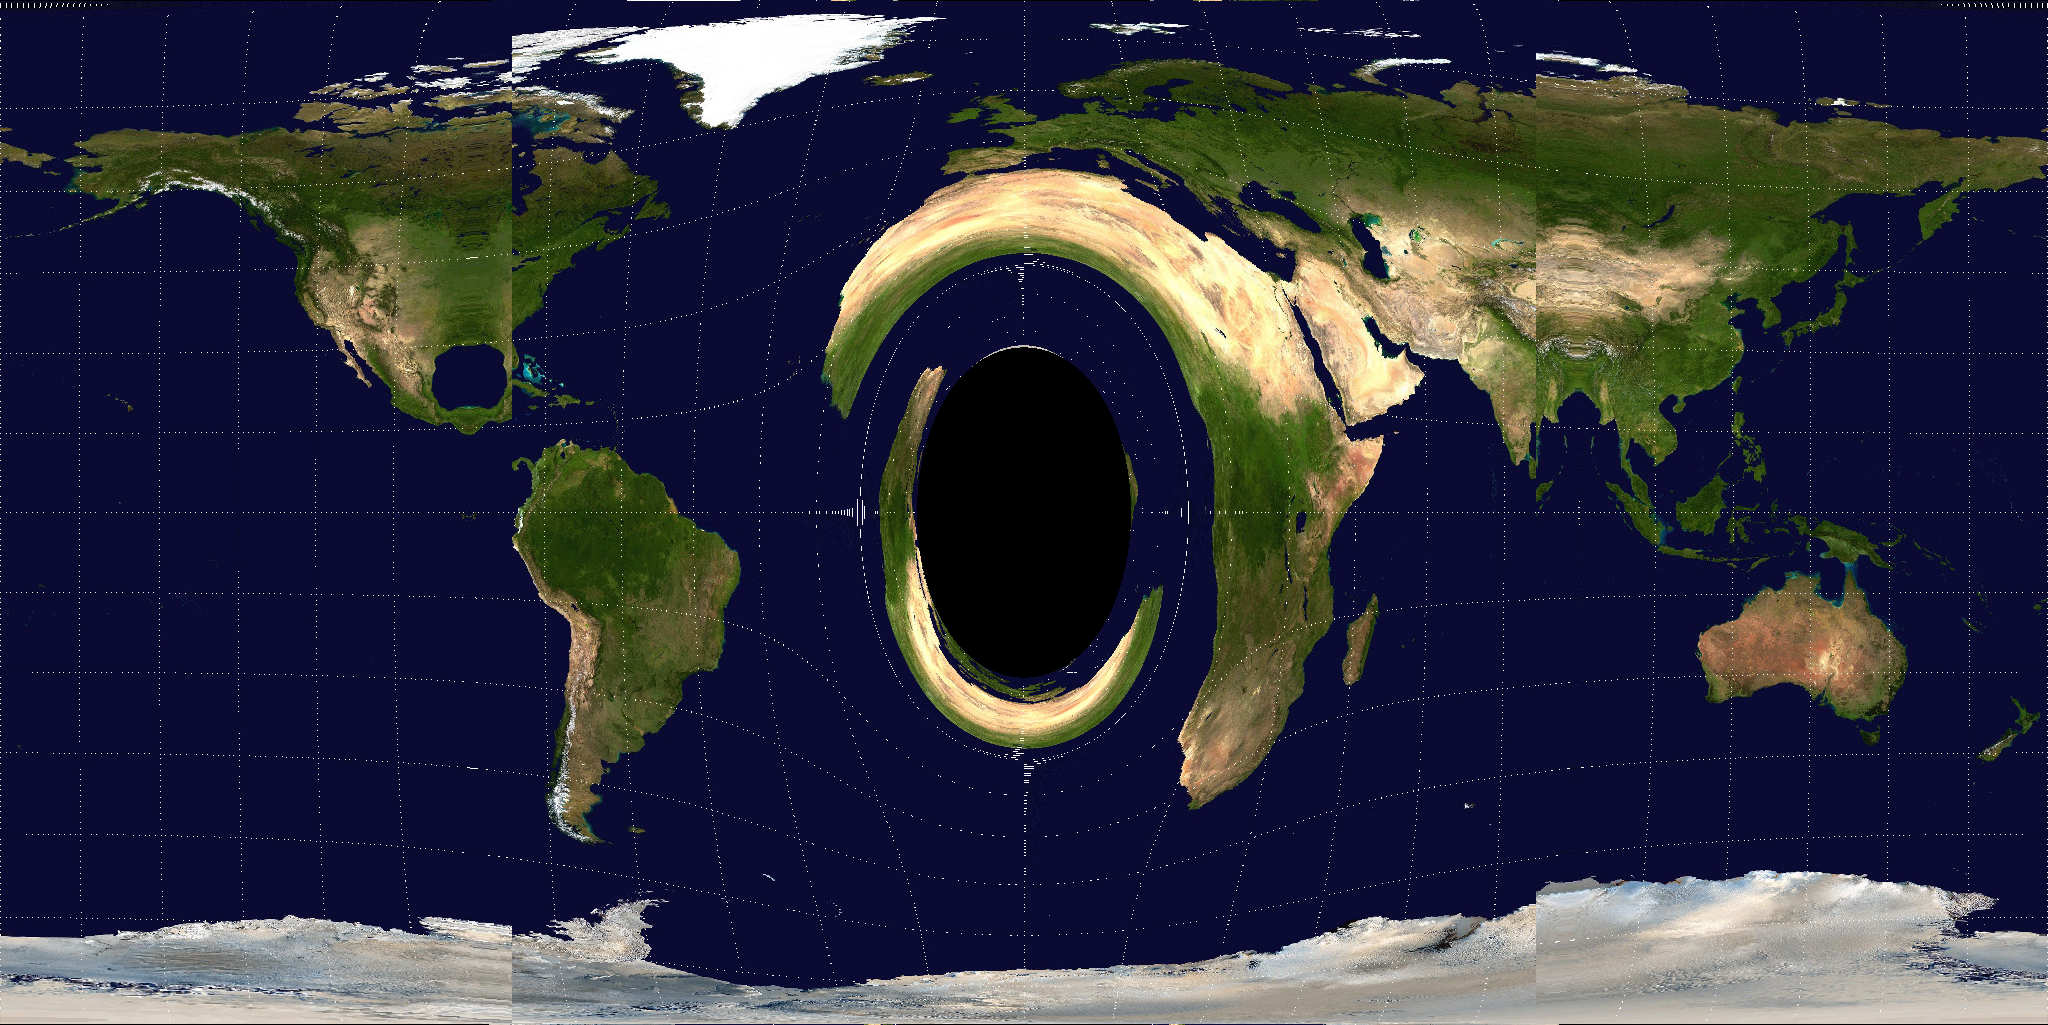
\includegraphics[width=\textwidth]{example_lens1}
\end{figure*}

\begin{figure*}
  \caption{\label{fig:example2}
    Second example of a generated Schwarzschild lensing map using the same space-time as in Fig.~(\ref{fig:example1}) but at a radius of $R_O=\SI{2.5}{\kilo\meter}$, which is significantly closer to the event horizon.
  }
  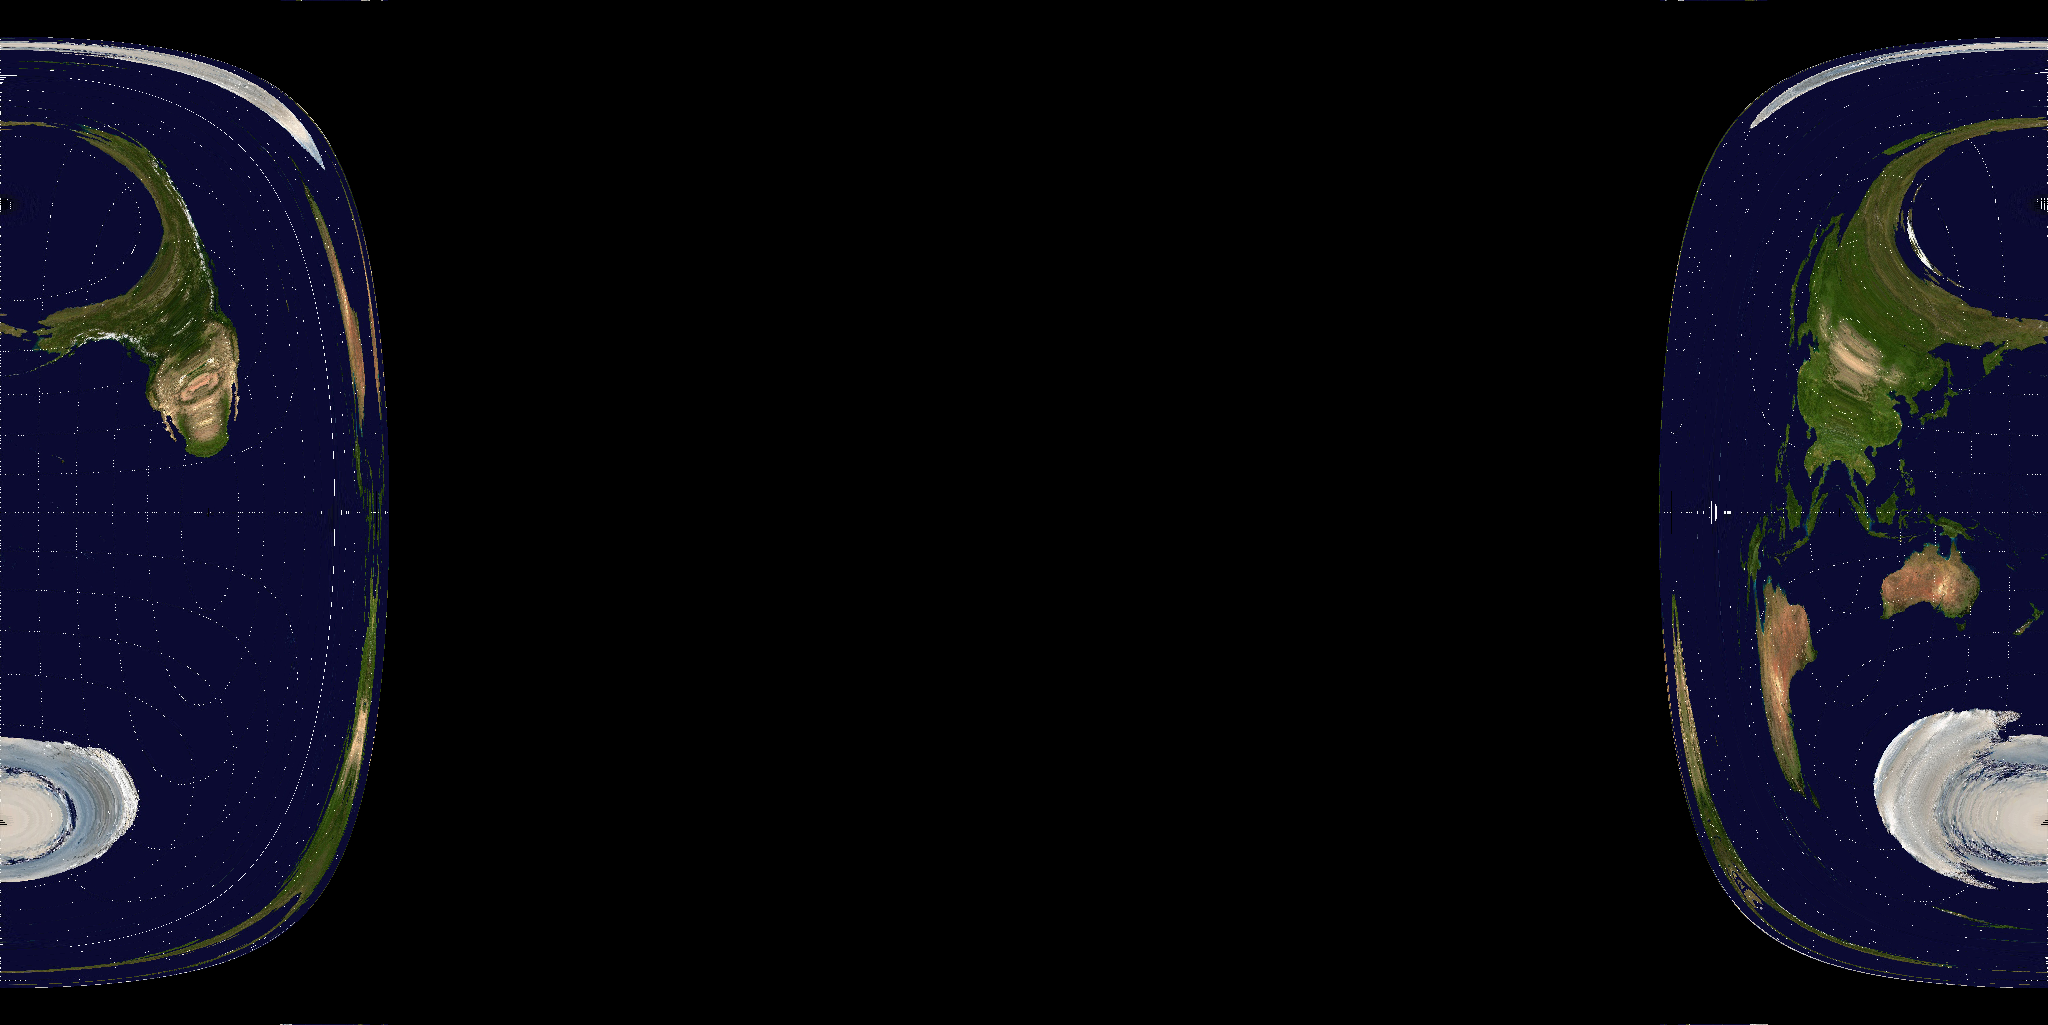
\includegraphics[width=\textwidth]{example_lens2}
\end{figure*}

\begin{figure*}
  \caption{\label{fig:lenscomparison}
    Comparison between the three levels of approximation in the Schwarzschild lensing equation.
    The first graph indicates the differences near the singularity, while the latter shows that the amount of error decreases significantly as the radius of the observer increases.
  }
  \begin{tabular}{c}
    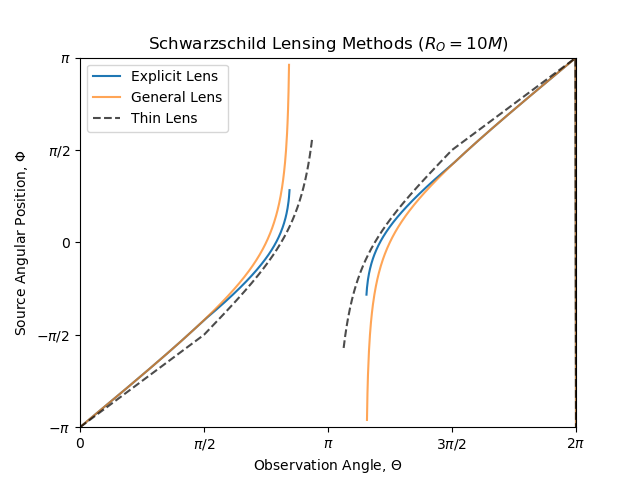
\includegraphics[width=.75\textwidth]{sc_lensing_near}\\
    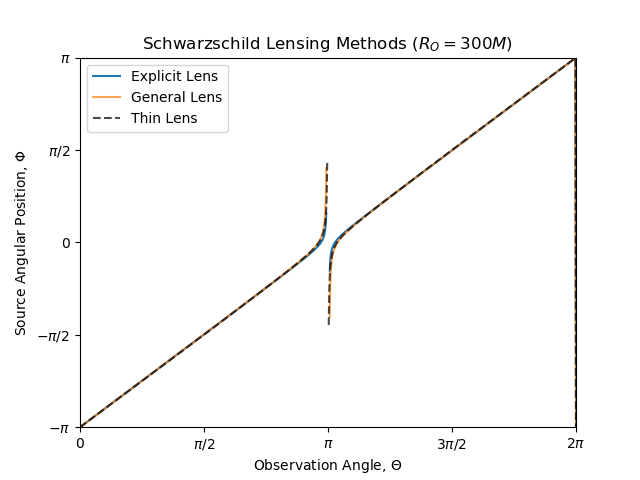
\includegraphics[width=.75\textwidth]{sc_lensing_far}
  \end{tabular}
\end{figure*}

\end{document}
